\documentclass[conference]{IEEEtran}
\IEEEoverridecommandlockouts
% The preceding line is only needed to identify funding in the first footnote. If that is unneeded, please comment it out.
\usepackage{cite}
\usepackage{amsmath,amssymb,amsfonts}
\usepackage{algorithmic}
\usepackage{graphicx}
\usepackage{textcomp}
\usepackage{xcolor}
\graphicspath{{./Screenshots}}

\def\BibTeX{{\rm B\kern-.05em{\sc i\kern-.025em b}\kern-.08em
    T\kern-.1667em\lower.7ex\hbox{E}\kern-.125emX}}
\begin{document}

\title{Towards Robust Federated Learning using Knowledge Distillation Techniques\\}

\author{\IEEEauthorblockN{Arindam Jain}
\IEEEauthorblockA{School of Computing \& Augmented Intelligence \\
Arizona State University \\
ajain243@asu.edu}
\and
\IEEEauthorblockN{Kiran Sthanusubramonian}
\IEEEauthorblockA{School of Computing \& Augmented Intelligence \\
Arizona State University \\
ksthanus@asu.edu}
}
\maketitle

\section{Introduction}
With the onset of improved privacy standards, edge computing capabilities, and large-scale machine learning requirements, Federated Learning has emerged as a privacy-preserving training paradigm for localized devices without data-sharing and aggregation requirements. With privacy-preserving benefits, users of these localized devices (e.g., mobile phones) also benefit from lower latencies in terms of required responses. Potential Federated Learning applications include improved mobile computing \cite{b1}, healthcare \cite{b2}, and autonomous vehicles.

In this project, we explore the use of Knowledge Distillation (KD) to create highly accurate and robust Federated Learning paradigms. Knowledge Distillation is conceptualized as a model compression technique in which large models with complex architectures are used to train a single smaller model that can run on devices with lesser computational capabilities while still achieving comparable performance levels. The most common Knowledge Distillation architecture is the Teacher-Student architecture (Fig.1).

The rest of this proposal is arranged as follows: Section II will detail the findings of the Literature Survey (including potential shortcomings), Section III will highlight the Problem Statement, Section IV will discuss the Methodology (including execution plan, datasets to be used, and the metrics to evaluate \& validate the methodology), Section V will summarize the objectives and learning outcomes from this project.
\begin{figure}[htbp]
\centering
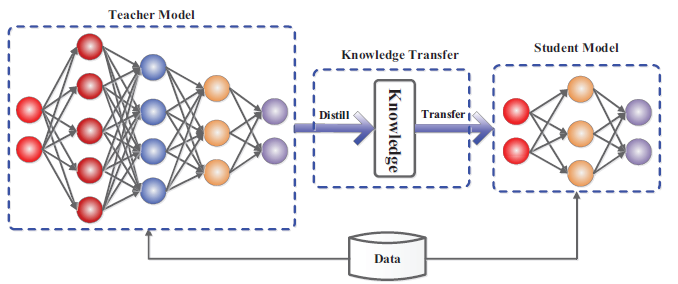
\includegraphics[scale=0.5]{Knowledge_Distillation.png}
\caption{Teacher-Student Architecture for Knowledge Distillation \cite{b3}}
\label{fig}
\end{figure}

\section{Literature Survey}
\subsection{Knowledge Distillation Techniques for Federated Learning}
One of the popular KD Algorithms for Heterogenous Federated Learning is proposed as FedMD (Li \& Wang) \cite{b4}. Here, the primary assumption is that our local nodes have the computation capability of defining and training their NN models specific to their local datasets - this helps solve the statistical heterogeneity of data across the nodes. FedMD focuses on utilizing the core idea of KD, i.e., using the Prediction Logits output from local Neural Network (NN) models averaged out as Knowledge to reach a better global consensus. FedMD also employs Knowledge Transfer (using a single giant global dataset) to overcome the issue of small local datasets. However, this paradigm is prone to Byzantine Faults and potential corruption of the global consensus due to adversarial attacks on one or more of the local nodes. Furthermore, the communication efficiency of the overall network architecture reduces as the number of nodes increases.

Related work to Robust Federated Learning is done in \cite{b5}, where several Client (Teacher) models are fused into a single Server (Student) model, which is further trained using unlabeled datasets to improve robustness. However, this does not defend against potential adversaries (a similar drawback to the algorithm presented in FedMD).

\subsection{Improving Fairness and Robustness of Federated Learning Architectures}
To improve Federated Learning architectures' fairness, accuracy, and robustness to potential Byzantine faults and adversarial attacks, we take inspiration from the algorithm proposed in Ditto (Tian Li et al) \cite{b6}. Here, personalization is used as a technique to balance robustness and fairness requirements. Personalization is mathematically conceptualized through regularization during local model updation with the global consensus calculated. The regularized parameter is tuned with respect to several factors, such as local dataset sample size, number of nodes affected by adversarial attacks, etc.

This paper also introduces essential robustness and fairness metrics, a crucial step toward defining evaluation parameters for Federated Learning research in real-world scenarios.

\begin{figure}[htbp]
\centering
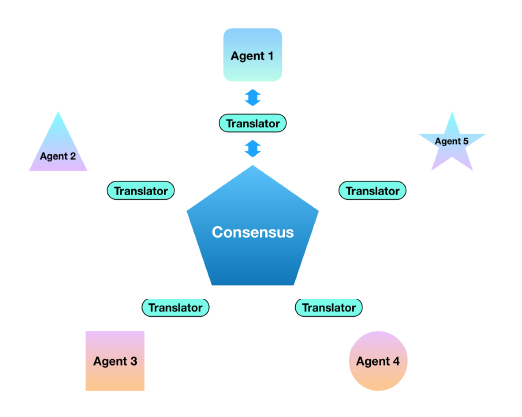
\includegraphics[scale=0.75]{Federated_Learning.png}
\caption{Heterogenous Federated Learning \cite{b4}. Here, the Translator is implemented using Knowledge Distillation in the FedMD Algorithm}
\label{fig}
\end{figure}

\section{Problem Statement}
Our problem statement is to increase the robustness of Knowledge Distillation techniques for Federated Learning. We intend to combine the idealogy presented in the FedMD algorithm with the Ditto Personalization Algorithm. We will define this combined implementation as a baseline for further investigating the effect of different Knowledge Distillation techniques, such as Ensemble, Cross-Modal \& Data-Free Distillation, to design robust, accurate \& communication-effective Federated Learning paradigms.   
\section{Methodology}
\subsection{Execution Plan}
Our plan of action can be broken down into the following stages:
\begin{enumerate}
\item Gain a Complete Theoretical \& Practical Understanding of Knowledge Distillation - specific to the Multi-Teacher to Student Architecture. (12.5\%)
\item Gain a Complete Theoretical \& Practical Understanding of general Federated Learning Paradigms such as FedAvg \cite{b7}. (12.5\%)
\item Implement the FedMD Algorithm for applying Knowledge Distillation to Federated Learning settings. (25\%)
\item Integrate the Ditto Algorithm step for Personalized Regularization to the created FedMD Algorithm. (20\%).
\item Simulate Adversarial attacks on a randomized node selection to verify the overall robustness (test accuracy) \& fairness of the network. Code \& visualize the evaluation metrics. FedMD + Ditto will be defined as a baseline implementation for other experiments. (20\%)
\item Integrate the Ditto Algorithm Personalization technique to any one of the other Knowledge Distillation techniques - Ensemble Distillation Algorithm, Cross-Modal, or Data-Free Distillation. (10\%)
\end{enumerate}

\subsection{Datasets}
We strictly define our problem space to Image Classification tasks. Implementing the FedMD algorithm requires a general public dataset \& local private datasets. The public/local dataset combinations will be Fashion MNIST/FEMNIST \& CIFAR10/subsets of CIFAR100. 
\subsection{Evaluation Metrics}
We will use the same evaluation metrics in the Ditto paper \cite{b6}. The robustness of the overall algorithm can be measured in terms of test accuracy in adversarial settings. Fairness can be measured in terms of test accuracy variance across several simulations. The comparison of evaluation metrics to related works will be based on the results provided in the Ditto paper.

\section{Objectives \& Learning Outcomes}


\begin{thebibliography}{00}
\bibitem{b1} W. Y. B. Lim et al., "Federated Learning in Mobile Edge Networks: A Comprehensive Survey," in IEEE Communications Surveys \& Tutorials, vol. 22, no. 3, pp. 2031-2063, third quarter 2020.
\bibitem{b2} Xu, J., Glicksberg, B.S., Su, C. et al. "Federated Learning for Healthcare Informatics," J Healthc Inform Res 5, 1–19 (2021).
\bibitem{b3} Gou, J., Yu, B., Maybank, S.J. et al. "Knowledge Distillation: A Survey." Int J Comput Vis 129, 1789–1819 (2021).
\bibitem{b4} Li, Daliang and Junpu Wang. “FedMD: Heterogenous Federated Learning via Model Distillation.” ArXiv abs/1910.03581 (2019)
\bibitem{b5} Tao Lin, Lingjing Kong, Sebastian U. Stich, and Martin Jaggi. 2020. "Ensemble distillation for robust model fusion in federated learning." In Proceedings of the 34th International Conference on Neural Information Processing Systems (NIPS'20). Curran Associates Inc., Red Hook, NY, USA, Article 198, 2351–2363.
\bibitem{b6} Tian Li, Shengyuan Hu, Ahmad Beirami \& Virginia Smith. (2021). "Ditto: Fair and Robust Federated Learning Through Personalization." 
\bibitem{b7} McMahan, H.B., Moore, E., Ramage, D., Hampson, S., \& Arcas, B.A. (2017). "Communication-Efficient Learning of Deep Networks from Decentralized Data." AISTATS.
\end{thebibliography}

\end{document}